\documentclass[12pt]{article}
\usepackage[paperwidth=24cm,paperheight=26.3cm,margin=0cm]{geometry}
\usepackage{fontspec}
\usepackage{xcolor}
\usepackage{tikz}
\usetikzlibrary{arrows.meta}
\pagestyle{empty}
\setlength{\parindent}{0pt}
\setmainfont{Times New Roman}

\definecolor{BrandBlue}{HTML}{005496}
\definecolor{FlowGreen}{HTML}{2E7D32}
\definecolor{FlowOrange}{HTML}{B26A00}
\definecolor{FlowGray}{HTML}{4B5563}
\definecolor{LightBlue}{HTML}{EAF3FB}
\definecolor{LightGreen}{HTML}{ECF7EE}
\definecolor{LightOrange}{HTML}{FFF4E2}
\definecolor{LightGray}{HTML}{F3F4F6}
\definecolor{LineColor}{HTML}{475569}
\definecolor{BorderColor}{HTML}{94A3B8}
\definecolor{TextColor}{HTML}{1F2937}
\definecolor{MutedText}{HTML}{6B7280}

\newcommand{\layerbox}[7]{%
	\draw[rounded corners=6pt, fill=#4, draw=BorderColor, line width=0.9pt] (#1,#2) rectangle (#3,#5);
	\draw[rounded corners=6pt, fill=#6, draw=#6, line width=0.9pt] (#1,#2) rectangle (#3,#2-0.62);
	\fill[#6] (#1,#2-0.46) rectangle (#3,#2-0.62);
	\node[anchor=west, text=white, font=\bfseries\fontsize{14}{16}\selectfont] at (#1+0.28,#2-0.32) {#7};
}

\newcommand{\boxtext}[5]{%
	\node[anchor=north west, align=left, text width=#3, text=TextColor, font=\fontsize{12.5}{14.5}\selectfont] at (#1,#2) {#4};
}

\newcommand{\centerbody}[4]{%
	\node[anchor=center, align=center, text width=#3, text=TextColor, font=\fontsize{11.5}{13.2}\selectfont] at (#1,#2) {#4};
}

\begin{document}
\noindent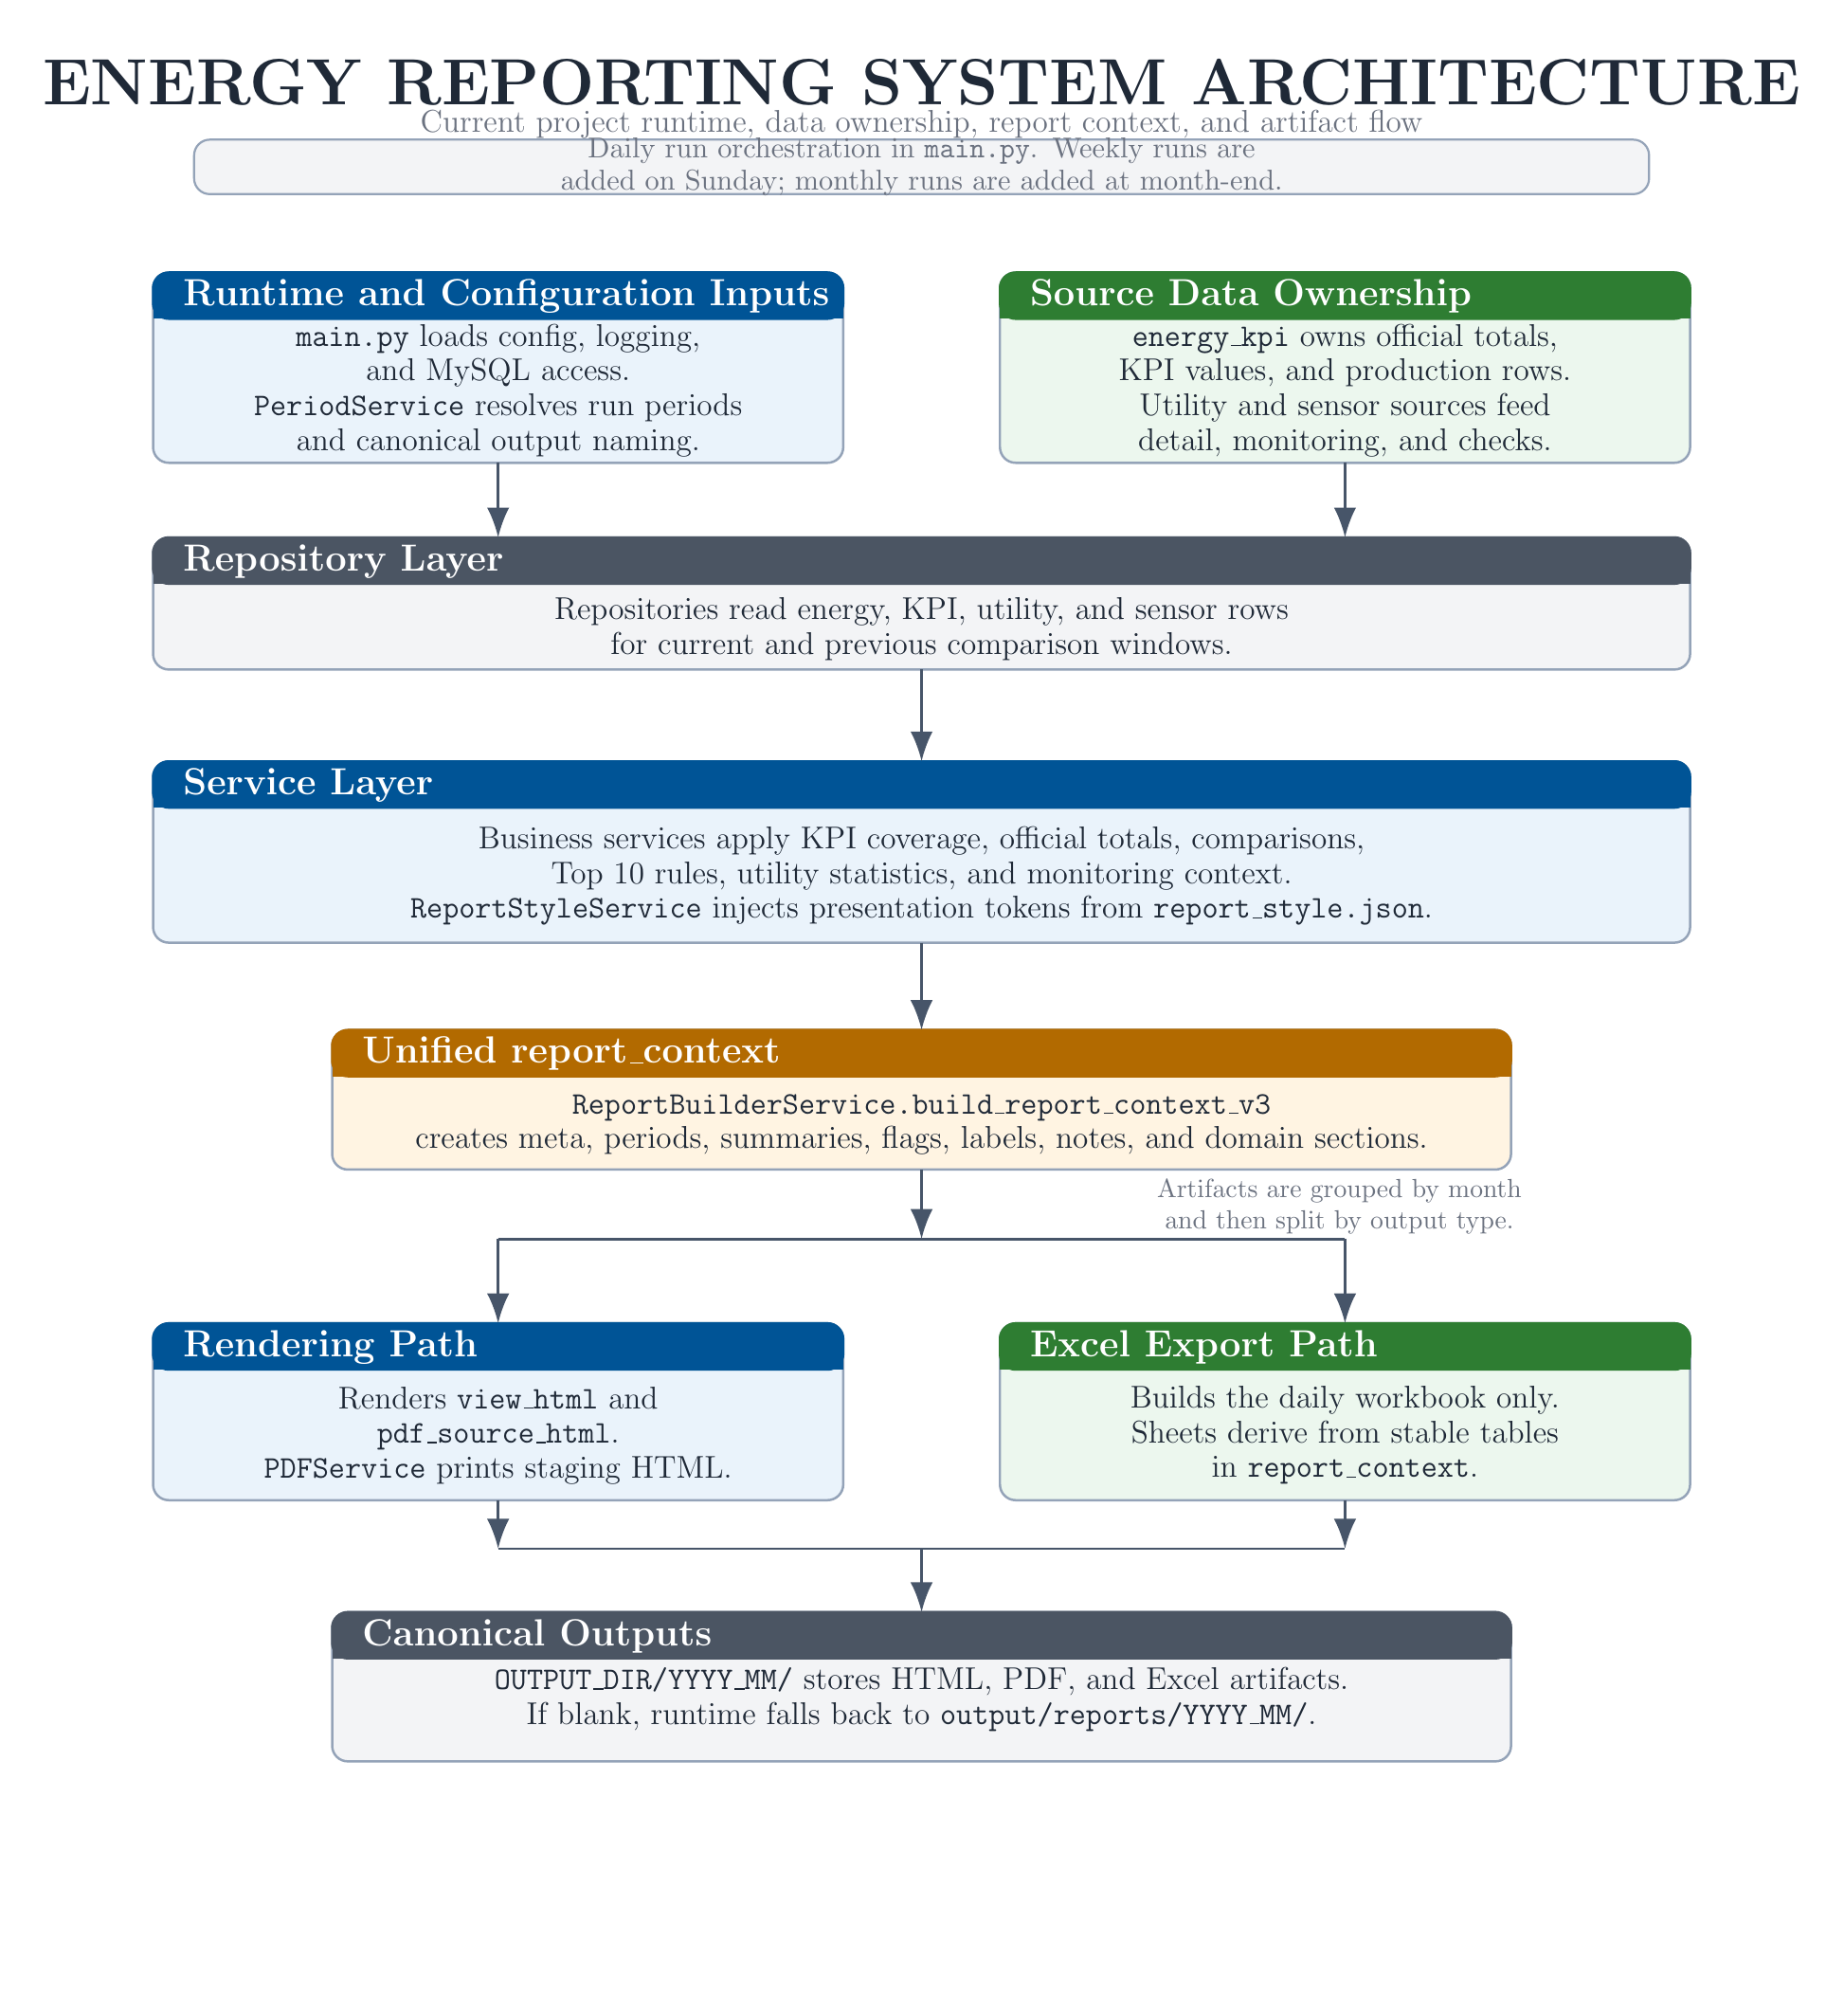
\begin{tikzpicture}[x=1cm,y=1cm]
	\fill[white] (0,0) rectangle (24,26.3);

	\node[font=\bfseries\fontsize{25}{28}\selectfont, text=TextColor] at (12,25.55) {ENERGY REPORTING SYSTEM ARCHITECTURE};
	\node[align=center, text width=16.8cm, font=\fontsize{12.5}{14.5}\selectfont, text=MutedText] at (12,24.98) {Current project runtime, data ownership, report context, and artifact flow};

	\draw[rounded corners=6pt, fill=LightGray, draw=BorderColor, line width=0.8pt] (2.25,24.05) rectangle (21.75,24.78);
	\node[anchor=center, align=center, text width=18.5cm, text=MutedText, font=\fontsize{10.5}{12.5}\selectfont] at (12,24.415) {Daily run orchestration in \texttt{main.py}. Weekly runs are added on Sunday; monthly runs are added at month-end.};

	% Top ownership and configuration inputs
	\layerbox{1.70}{23.00}{10.95}{LightBlue}{20.45}{BrandBlue}{Runtime and Configuration Inputs}
	\centerbody{6.325}{21.42}{8.45cm}{%
		\texttt{main.py} loads config, logging,\\and MySQL access.\\
		\texttt{PeriodService} resolves run periods\\and canonical output naming.}

	\layerbox{13.05}{23.00}{22.30}{LightGreen}{20.45}{FlowGreen}{Source Data Ownership}
	\centerbody{17.675}{21.42}{8.45cm}{%
		\texttt{energy\_kpi} owns official totals,\\KPI values, and production rows.\\
		Utility and sensor sources feed\\detail, monitoring, and checks.}

	% Repository and service layers
	\layerbox{1.70}{19.45}{22.30}{LightGray}{17.68}{FlowGray}{Repository Layer}
	\centerbody{12}{18.22}{19.10cm}{%
		Repositories read energy, KPI, utility, and sensor rows\\for current and previous comparison windows.}

	\layerbox{1.70}{16.45}{22.30}{LightBlue}{14.02}{BrandBlue}{Service Layer}
	\centerbody{12}{14.91}{19.10cm}{%
		Business services apply KPI coverage, official totals, comparisons,\\Top 10 rules, utility statistics, and monitoring context.\\
		\texttt{ReportStyleService} injects presentation tokens from \texttt{report\_style.json}.}

	% Unified context
	\layerbox{4.10}{12.85}{19.90}{LightOrange}{10.98}{FlowOrange}{Unified report\_context}
	\centerbody{12}{11.58}{14.90cm}{%
		\texttt{ReportBuilderService.build\_report\_context\_v3}\\creates meta, periods, summaries, flags, labels, notes, and domain sections.}

	% Output paths
	\layerbox{1.70}{8.92}{10.95}{LightBlue}{6.55}{BrandBlue}{Rendering Path}
	\centerbody{6.325}{7.42}{8.45cm}{%
		Renders \texttt{view\_html} and\\\texttt{pdf\_source\_html}.\\
		\texttt{PDFService} prints staging HTML.}

	\layerbox{13.05}{8.92}{22.30}{LightGreen}{6.55}{FlowGreen}{Excel Export Path}
	\centerbody{17.675}{7.42}{8.45cm}{%
		Builds the daily workbook only.\\
		Sheets derive from stable tables\\
		in \texttt{report\_context}.}

	\layerbox{4.10}{5.05}{19.90}{LightGray}{3.05}{FlowGray}{Canonical Outputs}
	\centerbody{12}{3.88}{14.90cm}{%
		\texttt{OUTPUT\_DIR/YYYY\_MM/} stores HTML, PDF, and Excel artifacts.\\If blank, runtime falls back to \texttt{output/reports/YYYY\_MM/}.}

	% Connectors
	\draw[-{Latex[length=4mm,width=3mm]}, line width=1.05pt, draw=LineColor] (6.325,20.45) -- (6.325,19.45);
	\draw[-{Latex[length=4mm,width=3mm]}, line width=1.05pt, draw=LineColor] (17.675,20.45) -- (17.675,19.45);
	\draw[-{Latex[length=4mm,width=3mm]}, line width=1.05pt, draw=LineColor] (12,17.68) -- (12,16.45);
	\draw[-{Latex[length=4mm,width=3mm]}, line width=1.05pt, draw=LineColor] (12,14.02) -- (12,12.85);
	\draw[-{Latex[length=4mm,width=3mm]}, line width=1.05pt, draw=LineColor] (12,10.98) -- (12,10.05);
	\draw[line width=1.05pt, draw=LineColor] (6.325,10.05) -- (17.675,10.05);
	\draw[-{Latex[length=4mm,width=3mm]}, line width=1.05pt, draw=LineColor] (6.325,10.05) -- (6.325,8.92);
	\draw[-{Latex[length=4mm,width=3mm]}, line width=1.05pt, draw=LineColor] (17.675,10.05) -- (17.675,8.92);
	\node[anchor=center, align=center, text width=8.8cm, text=MutedText, font=\fontsize{10}{12}\selectfont] at (17.60,10.48) {Artifacts are grouped by month\\and then split by output type.};
	\draw[line width=1.05pt, draw=LineColor] (6.325,5.90) -- (17.675,5.90);
	\draw[-{Latex[length=4mm,width=3mm]}, line width=1.05pt, draw=LineColor] (6.325,6.55) -- (6.325,5.90);
	\draw[-{Latex[length=4mm,width=3mm]}, line width=1.05pt, draw=LineColor] (17.675,6.55) -- (17.675,5.90);
	\draw[-{Latex[length=4mm,width=3mm]}, line width=1.05pt, draw=LineColor] (12,5.90) -- (12,5.05);
\end{tikzpicture}
\end{document}
